\documentclass{article}
%\usepackage[a4paper, total={6in, 8in}]{geometry}
\usepackage{geometry}
 \geometry{
 a4paper,
 total={210mm,297mm},
 left=20mm,
 right=20mm,
 top=-2mm,
 bottom=2mm,
 }
%\usepackage[margin=0.5in]{geometry}

\usepackage{amsmath,amssymb}
\usepackage{ifpdf}
%\usepackage{cite}
\usepackage{algorithmic}
\usepackage{array}
\usepackage{mdwmath}
\usepackage{pdfpages}
\usepackage{mdwtab}
\usepackage{eqparbox}
\usepackage{cite}
%\onecolumn
%\input{psfig}
\usepackage{color}
\usepackage{graphicx}
\setlength{\textheight}{23.5cm} \setlength{\topmargin}{-1.05cm}
\setlength{\textwidth}{6.5in} \setlength{\oddsidemargin}{-0.5cm}
\renewcommand{\baselinestretch}{1}
\pagenumbering{arabic}
\usepackage{ragged2e}
\renewcommand{\baselinestretch}{1.5}

\begin{document}

\textbf{
\begin{center}
{
\large{School of Engineering and Applied Science (SEAS), Ahmedabad University}\vspace{4mm}
}
\end{center}
%
\begin{center}
\large{B.Tech(ICT) Semester IV: Probability and Random Processes (MAT 202) }\\ \vspace{3mm}
\end{center}
}
\begin{itemize}
\item Group No : \textbf{S\textunderscore B1}
\item Name (Roll No) :  \textbf{Nancy Radadia(AU1841070), Suhanee Patel(AU1841113), Yash Patel(AU1841125) }

\item Project Title: \textbf{Prediction of the Probabilities of the Transmission
	of Genetic Traits within Bayesian Logical Inference}

\end{itemize} 

\section{Introduction}
\subsection{Background}
\begin{itemize}
    \item Have you ever noticed that some of us might resemble our parents in some way? Like we might have matching eye colour, or similar hair textures etc. We got these characteristics from our parents, and they got them from their parents. So eventually we can say that these biological informations are passed from one generation to another. These units of inheritance are known as traits. Here we aim to predict the traits in future generations provided the data of past generations. By using some probabilistic modelling we can predict the probability of transmission of genetic traits.   	
    
    \item There are many models designed to study the phenotypic prediction of traits at individual levels such as eye color \cite{hart2013improved}, height\cite{dubois2012genetic} ,hair color, skin color \cite{liu2015genetics} etc. Prediction of traits is used for many purposes like quantifying the risks of diseases for individuals\cite{mclaren2016privacy} \cite{yi2011bayesian} \cite{wijeysundera2011predicting} \cite{farrer1997effects} . Diseases can be of different types. Among which one in autosomal recessive disease. Such diseases are transmitted when an infected recessive gene is crossed with another infected recessive gene . When a mutated gene from both parents is passed to their child then that child is said to be affected. We can model different and complex scenarios using appropriate probabilistic models to find the required likelihoods and estimate the risks accordingly \cite{ogino2004bayesian}. 
    \item Prediction of  an autosomal recessive disease named Cystic Fibrosis(CF)\cite{drumm2012genetic} is demonstrated in our base article. Cystic Fibrosis(CF) is a single-gene disorder caused by mutations in CF transmembrane conductance regulator (CFTR) genes found in cells that line the lungs, digestive tract, sweat glands, and genitourinary system. CF patients are expected to die within the first years of life. Their life expectancy has lengthened with advances in diagnosis and treatment and is currently about 38 years \cite{jackson2011validation}. 
    
\end{itemize}

\subsection{Motivation}
\begin{itemize}
	\item The main vision behind this study is to be able to predict the genetic traits in future generations from the data of the prior generation. This prediction can serve extremely helpful for understanding the risks of any diseases which could be passed by inheritance. Once predicted, suitable precautionary measures can be taken. This can increase the recovery chances of individuals and improve the overall life expectancy. So if we are able to know any information related to genetic traits of our future generations, we have a chance to take prior actions.
\end{itemize}
\subsection{Problem Statement/ Case Study}
     Our base article aimed at calculating the probability of a heterozygous offspring based on the data and information provided by the previous generations and by taking some prior assumptions. We have derived a general formula for finding the probability for a mono hybrid genetic cross and have generated a matlab code to verify our results with those given in the article. We have used Bayesian logical inferences along with Markov chain to model the uncertainty. The final aim of the article was to predict autosomal recessive diseases for evaluating its performance on real-world data under Bayesian framework. Also in order to demonstrate and evaluate the flexibility of the method, we have tried to evaluate different examples of pedigree diagrams and punnett squares which contain different genetic crosses, such as monohybrid, dihybrid, trihybrid and multi hybrid genetic crosses and have came to a general formula using which we can find the probability upto 'n' number of generations and analyzing  'm' number of traits. 
\section{Data Acquisition }

\begin{itemize}
    \item The example which we worked on dont require any data set, as we are taking some assumptions for the past generations and trying to model it to derive a general formula for different scenarios for the nth generation.        
\end{itemize}
%are Once accomplished,we can improve sensing performance based on  the knowledge of channel statistics. Further, for more realistic considerations we would extend the above setup to SIMO, MISO and MIMO system models. The performance metrics would be the statistical properties like idle/busy period durations, its mean, variance and Occupancy rate(or duty cycle) of Primary user (PU). The metric for spectrum sensing would be detection probability $(P_d).$ Also the estimation error varies as per sensing period$(T_s)$ and thus KS distance would be an additional metric to be taken into consideration. 
	%\vspace{8cm}
\section {Probabilistic Model Used/ PRP Concept Used}

\subsection{Methodolgy/Appraoch}

\begin{itemize}
 
\item The very first goal of the probabilistic model here is to analyse inheritance of traits in human and animal populations. It then determines the mode of inheritance such as \textbf{dominant} or \textbf{recessive}. This can be achieved by the use of \textbf{pedigree analysis} which describes the characteristics of all the generations in a family.\\
The next goal is to calculate the probability of an affected offspring for a given genetic cross. To achieve this there are various methods but here in this model we use \textbf{Bayesian logical inferences}.\\
Also, the outcome of genetic crossing of traits depends only on that of the previous one which can be known from pedigree analysis and is used to create transmission probability vector of traits for a given generation. A special kind of stochastic process called \textbf{Markov chain} uses this vector to predict posterior probability of transmission of genetic traits under some assumptions. Hence we calculate the probability of an affected offspring among generations within \textbf{Bayesian framework with Markov chain}. Also, using this probabilistic model we can even predict transmission of hereditary diseases among generations such as Cystic fibrosis (CF).
\end{itemize} 

\subsection{Bayesian logical inferences}
\begin{itemize}

\item The task of Bayesian logical inferences here is to infer the probability for the hypothesis \textbf{H}, given some data \textbf{D} from experiment and capturing all relevant information \textbf{I}. This
can be done within the setting of Bayes’ theorem which states  
\begin{align*}      
Pr(H|D,I) = \dfrac{Pr(D|H,I)\cdot Pr(H|I)}{Pr(D|I)} 
\end{align*} 
Here, $ 	Pr(D|I) $ is is a global likelihood for entire class of \textbf{H} or evidence given some information \textbf{I}. The quantity $ Pr(D|H,I) $ is called likelihood of H, which measures or determines a probability of observations D, or the statistic under the hypothesis being tested. The quantity $ Pr(H|I) $ is known as a prior probability distribution function (PDF) of H in the absence of D and the quantity $ Pr(H|D,I) $ is a posterior PDF of H. 
\end{itemize}

\subsection{Pedigree Analysis and Modelling for monohybrid crosses}
\begin{itemize}
	\item To study Pedigree Analysis for Monohybrid crossess, consider an example of hamster and we suppose that a single gene controls the hair length of a hamster. Then, a short hair is governed by a dominant gene and represented by \textbf{\textit{L}} while a long hair is governed by a recessive gene and represented by \textbf{\textit{l}}. Therefore, a hamster will be phenotypically short haired unless its genotype is (\textit{ll}). Consider the given figure which represents the pedigree analysis of monohybrid genetic crosses. Also, in  \textit{$ G_1 $} both parents are known to be phenotypically short haired. Crossing of \textit{(Ll)} and \textit{(LL)} is given in figure 2-\\
	\pagebreak
	 \begin{figure}[h]
		\centering
		\begin{minipage}[b]{0.32\textwidth}
            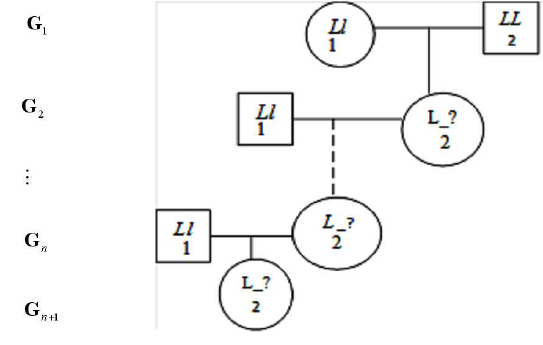
\includegraphics[width=1.2\textwidth]{monohybrid_pedigree}
			\caption{Pedigree diagram for monohybrid crosses of $ G(n+1)_2 $}
		\end{minipage}%
		\hspace{3cm}
		\begin{minipage}[b]{0.32\textwidth}
			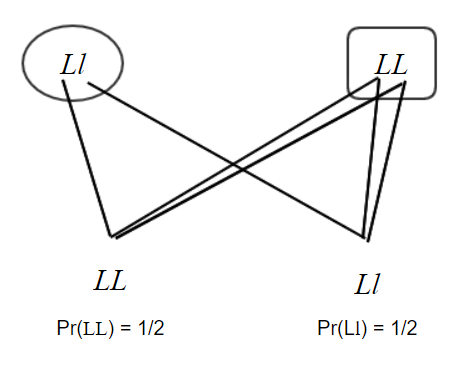
\includegraphics[width=1\textwidth]{a1}
			\caption{Genetic crossing of $ G_1 $ generation}
		\end{minipage}
	\end{figure}
  
  \item Hence, the probability of \textit{(LL)} = \textit{(Ll)} = 1/2 and both the outcomes ultimately turn out to be phenotypically short hair, where one is heterozygous short hair \textit{(Ll)} whereas another is homozygous short haired \textit{(LL)}. Given that $ G_{i1} $'s are carriers and $ G_{(n+1)2} $ has a short hair, we would like to find the probability of $ G_{(n+1)2} $ being genotypically heterozygous \textit{Ll}.\\
  To find the probability of the affected offspring we use bayesian method as discussed before. From the pedigree diagram we can say that our information \textbf{\textit{I}} represents that
  the genotypes of parent $ G_{11} $  and $ G_{12} $  are initially known to be heterozygous short haired \textit{(Ll)} and homozygous short haired \textit{(LL)} respectively and our evidence \textbf{\textit{E}} is that $ G_{i2} $ is short hair. Let us define H = {$ (h_{i})^{k}_{i=1} =$} \{\textit{Ll},\textit{Ll},\textit{ll}\} where k is the number of hypothesis. Now since we are finding the probability of h2 i.e. \textit{Ll}, the bayseian equation takes the following form:
  \begin{align*}      
  Pr(h_2|E,I) &= \dfrac{Pr(E|h_2,I)\cdot Pr(h_2|I)}{Pr(E|I)}\\\\
  &= \dfrac{Pr(E|h_2,I)\cdot Pr(h_2|I)}{\sum_{i=1}^{m}Pr(E|h_i,I)\cdot Pr(h_i|I)} \hspace{2cm} (1).
  \end{align*}\\
  The total probability in the denominator is calculated using Markov chain.
\end{itemize}

\section{Pseudo Code/ Algorithm }

\begin{itemize}
    \item To calculate the total probability in Eq.(1) we use matrices whose components indicate probabilities of genetic crosses of traits. In this context, a relationship between the probabilities of the offspring’s genotypes and that of its parents can be modeled using transition matrices used in the Markov chains. Therefore, the probability values of outcomes of genotypes by crossing $ G_{11} $ with \textit{LL}, \textit{Ll}, and \textit{ll} is shown in the figure below and then using this we form transition matrix A which is shown in table I.

    \begin{figure}[h]
    	\centering
    	\begin{minipage}[b]{0.32\textwidth}
    		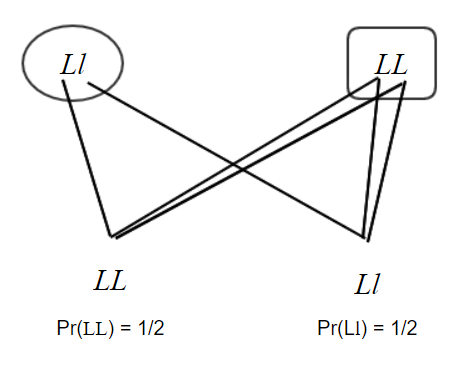
\includegraphics[width=1.2\textwidth]{a1}    		
    	\end{minipage}%
    	\hspace{3cm}
    	\begin{minipage}[b]{0.32\textwidth}
    		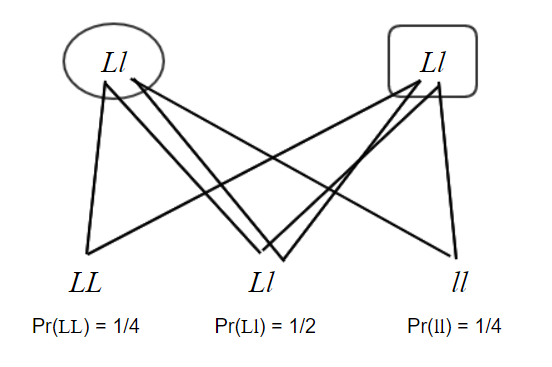
\includegraphics[width=1.3\textwidth]{a3}    	
    	\end{minipage}
    	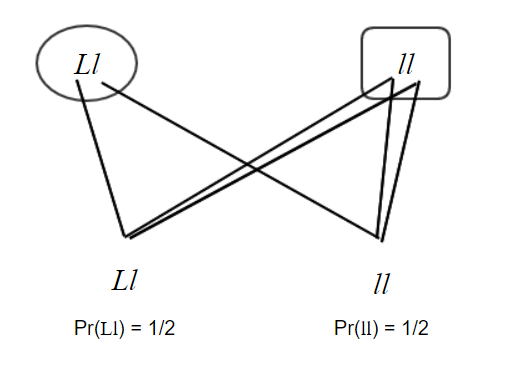
\includegraphics[height= 5cm ,width=7cm]{a2}               
    \end{figure}
     
    \begin{figure}[h]
    	\centering
    	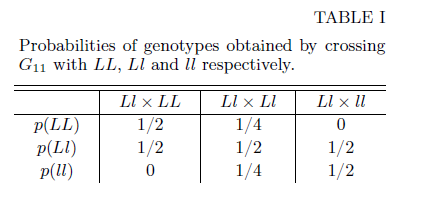
\includegraphics[height= 5cm ,width=10cm]{table}
    \end{figure} 
    Hence, from the figures obtained from genetic crossing of traits we get transition matrix A, shown in table I.
    
    \item On the other hand, let x represent the prior probabilities of hypothesis {$ (h_{i})^{k}_{i=1} =$} of genotypes \{\textit{Ll},\textit{Ll},\textit{ll}\} so that initially, $ x_0 = [1, 0, 0]^T $ because $ G_{12} $ is given as \textit{LL} genotype in Figure 1. After one generation,
    \begin{align*}
    x_1 = Ax_0 = [0.5, 0.5, 0]^T 
    \end{align*}
     Similarly, after two generations, 
    \begin{align*}
    x_2 = Ax_1 = A^2x_0 
    \end{align*}
    Hence after n generation where $ (n\in Z^+) $ we have 
    \begin{align*}
    x_n  = A^nx_0 
    \end{align*}
    Here it is required to calculate higher power of matrix A, hence we can use one of the linear algerbra property i.e. \textbf{Diagonalization}
    \begin{align*}
    x_n  = A^nx_0 = P\triangle^{n}P^{-1}x_0 
    \end{align*}	
    where $ \triangle $ is a diagonal matrix whose diagonal entries are eigenvalues of A and P is a matrix whose columns are linearly independent eigenvectors of A corresponding to its eigenvalues. To obtain the value of $ Pr(E|I) $ we multiply $ x_n $ ny normalisation constant d which is $ [1,1,0]^T $ as $ p(E|h1, I) = p(E|h2, I) $ = 1 and $ p(E|h3, I) $ = 0, respectively. Thus, going back to Eq.(1) we calculated $ Pr(E|I) $, also the value of $ Pr(h_2|I) = 1/2 $ and $ Pr(E|h_2,I) = 1 $. Hence, substituting all these values in Eq(1) we can calculate probablity of hetrozygous short hair of any given $ n^{th} $ generation.
    \item To derive general expression, we first calculate the probability of first few generations,
    After \textbf{first generation}, we calculate probability as follows
    \begin{align*}
    x_1 &= Ax_0 = [0.5, 0.5, 0]^T\\
    x_1 \cdot d &=  [1, 1, 0]\cdot[0.5, 0.5, 0]^T = 1 = p(E|I) 
    \end{align*}
    Substituting, the above value in equation (1), the probability for hetrozygous short hair after generation 1 will be
    \begin{align*}
    Pr(h_2|E,I) &= \dfrac{Pr(E|h_2,I)\cdot Pr(h_2|I)}{Pr(E|I)}\\\\
    &= \dfrac{1/2 \cdot 1}{1}\\
    Pr(h_2|E,I) &= \dfrac{1}{2}
    \end{align*}	
    Similarly, After \textbf{second generation}, we calculate as follows
    \begin{align*}
    x_2 &= A^2x_0 = [3/8, 1/2, 1/8]^T\\
    x_2 \cdot d &=  [1, 1, 0]\cdot[3/8, 1/2, 1/8]^T = 7/8 = p(E|I) 
    \end{align*}
    Substituting, the above value in equation (1), the probability for hetrozygous short hair after generation 2 will be
    \begin{align*}
    Pr(h_2|E,I) &= \dfrac{Pr(E|h_2,I)\cdot Pr(h_2|I)}{Pr(E|I)}\\\\
    &= \dfrac{1/2 \cdot 1}{7/8}\\
    Pr(h_2|E,I) &= \dfrac{4}{7}
    \end{align*}
    After, \textbf{Third generation},
    \begin{align*}
    x_3 \cdot d &=  [1, 1, 0]\cdot[5/16, 1/2, 3/16]^T = 13/16 = p(E|I)\\\\
    Pr(h_2|E,I) &= \dfrac{Pr(E|h_2,I)\cdot Pr(h_2|I)}{Pr(E|I)}\\\\
    Pr(h_2|E,I) &= \dfrac{8}{13}
    \end{align*}
    Observing the above trend in values for generation, we arrive at general form of equation -
    \begin{align*}
    Pr(h_2|E,I) &= \dfrac{1/2 \cdot 1}{\Big[1 + \Big(-\dfrac{1}{8}\Big) + \Big(-\dfrac{1}{16}\Big) +.......+ \Big(-\dfrac{1}{2^{n}}\Big)\Big]}
    \end{align*}
    for after n $ (n\in Z^+) $ generation.\\\\
    Solving the above equation further,\\ 
    \begin{align*}
    Pr(h_2|E,I) &= \dfrac{1/2 \cdot 1}{1 - \Big(\dfrac{1}{8} + \dfrac{1}{16} + \dfrac{1}{32} +......+ \dfrac{1}{2^{n}}\Big)}
    \end{align*}\\
    Solvoing the above denominator by using Geometric Progression, where a (first term) = 1/8 and r (difference) is 1/2. Formula for solving G.P. goes like this-
    \begin{align*}
    Sum &= \dfrac{a\cdot\Big(r^n - 1\Big)}{r - 1}\\\\
    &= \dfrac{1/8\cdot\Big(\dfrac{1}{2^n} - 1\Big)}{\dfrac{1}{2} - 1}
    \end{align*}
     Substituting in sum in the equation we get,
    \begin{align*}
    Pr(h_2|E,I) &= \dfrac{\dfrac{1}{2}\cdot 1}{1 - \Big(\dfrac{\dfrac{1}{8}\cdot\Big(\dfrac{1}{2^n} - 1\Big)}{-\dfrac{1}{2}}\Big) }\\\\
    &= \dfrac{1/2}{\dfrac{3}{4} + \dfrac{1}{2^{n+1}}}
    \end{align*}
     Multipling by $ 2^{n+1} $ on both numerator and denominator we get the final equation as-
    \begin{align*}
    \boxed{Pr(h_2|E,I) = \dfrac{2^n}{3\cdot 2^{n-1} + 1}}
    \end{align*}\\
    The above equation is the posterior PDF of $ h_2 $ i.e hetrozygous short hair \textit{(Ll)} after n generations for \textbf{Monohybrid Crosses}
     
    
    
 \end{itemize}



\section{Coding and Simulation} 
\subsection{Simulation Framework}
\justify We try to simulate the above derived equation for monohybrid crosses in matlab. The x-axis represent the generations and the the Y axis represents the probability of hetrozygous short hair in the correspoding generation of X-axis.
The transition matrix A, prior probability distribution i.e. $Pr(h_2|I) $ and $ Pr(E|h_2,I) $ are predefined and we calculate the total probability in the denominator and find the PDF for each generation. The no of generations will also be predefined and the no of times we calculate the total probability or the number of tumes we run Markov chain simulations depends on n (generation). We use for loop running from 0 to n which calculates simualtion of Total probability and calculates the PDF.
\subsection{Reproduced Figures}
\begin{itemize}
\item Here, we plot generation vs Posterior PDF of hetrozygous short hait \textit{(Ll)}, where we take n (no. of generation) = 20, hence we run for loop for 20 times and calculate PDF as shown below.\\
\begin{figure}[h]
	
	\begin{minipage}[b]{0.32\textwidth}
		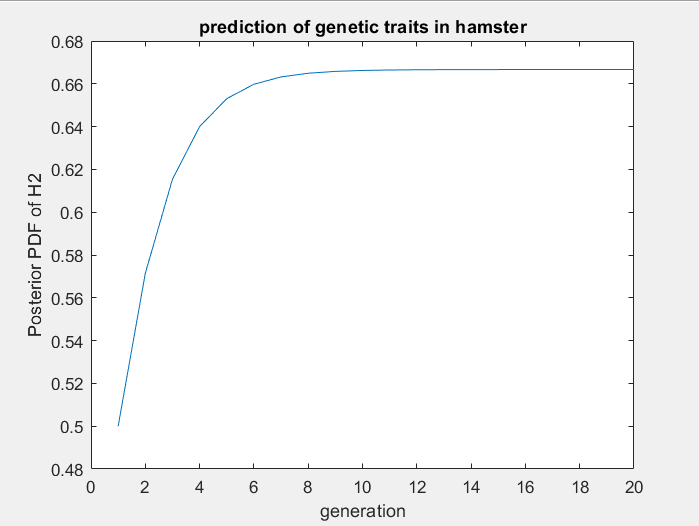
\includegraphics[width=1.5\textwidth]{code1}
		\caption{Posterior pdf for h2 \textit{(Ll)}}
	\end{minipage}%
	\hspace{3.5cm}
	\begin{minipage}[b]{0.32\textwidth}
		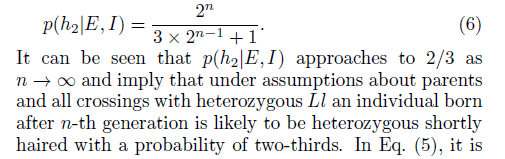
\includegraphics[width=1.5\textwidth]{compare}
		\caption{Results of PDF for h2 in base article}
	\end{minipage}%
	
	
	
	%	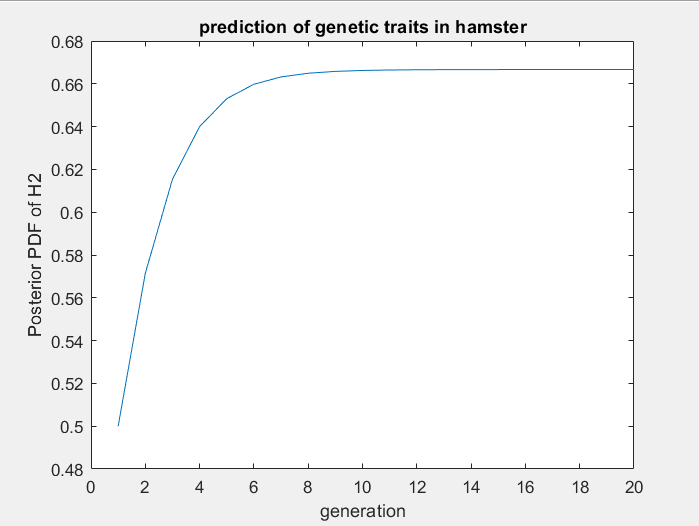
\includegraphics[height=7cm,width=9cm]{code1}
	%   \caption{Posterior pdf for h2 \textit{(Ll)}}    		
\end{figure}\\
Here, figure 4 is as per the article which states that as $ (n\rightarrow \infty),  Pr(h2|E,I) $ approaches 2/3 i.e. 0.66 which matches with our plot given in Figure 3.
\end{itemize}

\subsection{New Work Done}

\subsubsection{New Analysis}

	We derived a general expression and implemented mathametical code that calculates posterior probability of hypothesis of genetic crosses for monohybrid. Now we try to extened the study by finding probabililty of hetrozygous traits in Dihybrid and Tridybrid using different method called \textbf{Punnett Square} and we arrive deriving the general expression of finding probability in multihybrid crosses.
	\begin{itemize}
     \item   \textbf{Dihybrid Crosses}\\
     In genetics, a dihybrid cross is known as cross between two hybrid genes of parents that differ in two traits of particular interest. The genes are located on separate chromosomes, so the traits themselves are \textbf{unrelated}. Let there be two traits in hamster, one which controls fur color and second which controls hair style (curly or straight). As, we discussed previously, for each trait, there are dominant and recessive genes. The dominant fur color is black and represented by \textbf{\textit{B}}, while the recessive fur color is white and represented by \textbf{\textit{b}}, similarly in second trait the dominant hair style is curly represented by \textbf{\textit{C}} and recessive hairstyle is represented by \textbf{\textit{c}}. Consider the pedigree diagram of diybrid:\\
     \begin{figure}[h]
     	\centering
     	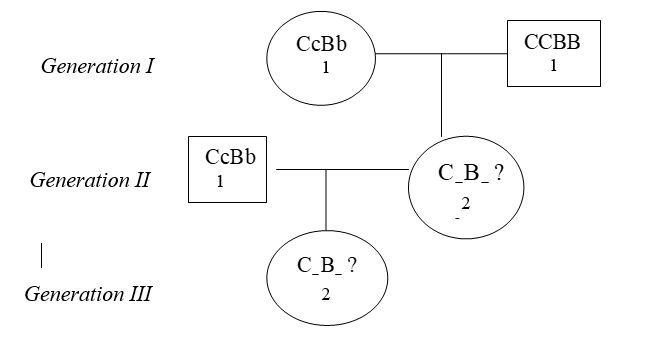
\includegraphics[height=5cm,width=9cm]{dihybrid_pedigree}
     	\caption{Genetic Pedigree for Dihybrid Cross}
     \end{figure}
     According, to figure 5, under the assumption that both Generation II-2 and III-2 are phenotypically curly haired and black fur, we try to find the probability of the Generation III-2 being genotypically heterozygous curly haired and black fur (CcBb). Genetic crossing of dhybrid is complexed as compared to monohybrid and hence we use a method called \textbf{Punnett square} for crossing.\\
    Since parents are heterozygous and homogeneous in a dihybrid cross, the possible gene combinations from each parent listed on the Punnett square are \textit{Bb}, \textit{BB}, \textit{Cc} and \textit{CC}. Given below are the punnet sqaure for both genertion II and generation III in table II and III respectively.
    \pagebreak
    \begin{figure}[h]
    	\centering
    	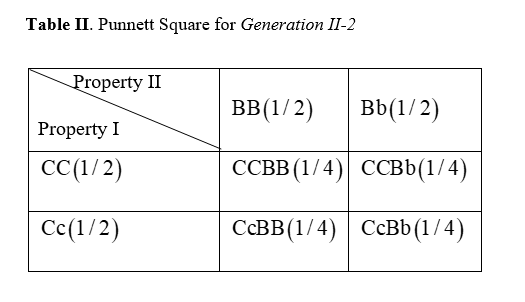
\includegraphics[height=5cm,width=9cm]{table2}
    \end{figure}\\
    From the above punnet square of Generation II, we can say that -\\
    
    	\hspace{4cm}$ Pr(h_2,I) = Pr(CcBb,I) = 1/4 $ \\
      
    \begin{figure}[h]
    	\centering
    	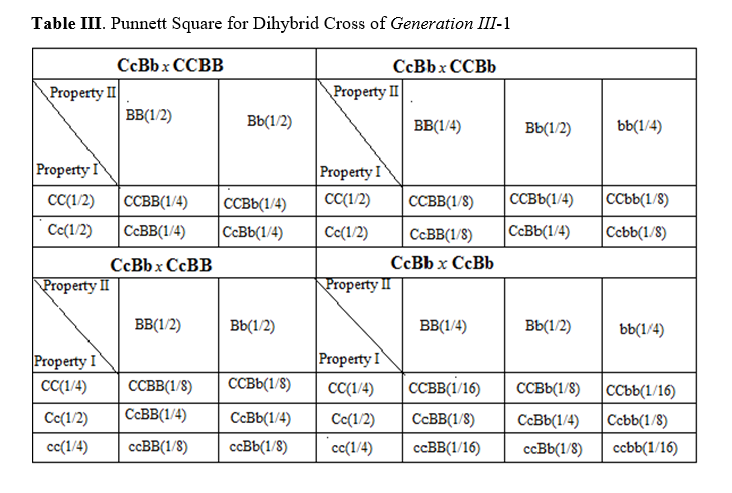
\includegraphics[height=9cm,width=12cm]{table3}
    \end{figure}
  To find the total probability in denominator of Equation (1):\\\\
  $ Pr(E|I) = Pr$(curly hair,black fur$| G$)\\
  $ Pr(E|I)$ = 1 - $ Pr $(straight hair,black fur \textbf{or} straight hair,white fur \textbf{or} curly\\ \hspace*{4cm} hair,while fur$| G$ ) \\\\
  $ Pr(E|I) = 1 - Pr(\{ccBb\},\{ccBB\},\{Ccbb\},\{CCbb\},\{ccbb\}| G)$\\\\
  From the punnett square of generation III, we can find the above probability:\\
  \begin{align*}
  Pr(E|I) &= 1 - \Big( \Big(\dfrac{1}{8} + \dfrac{1}{8}\Big)\cdot \dfrac{1}{4} + \Big(\dfrac{1}{8} + \dfrac{1}{8}\Big)\cdot\dfrac{1}{4} + \Big(\dfrac{1}{8} + \dfrac{1}{8} + \dfrac{1}{16} + \dfrac{1}{16} + \dfrac{1}{16}\Big)\cdot\dfrac{1}{4} \Big) \\\\
  Pr(E|I) &= 1 - \Big(\dfrac{15}{64}\Big)\\\\
  Pr(E|I) &= \dfrac{49}{64}       
  \end{align*}
  Now substituting the values in bayesian Equation (1) we get the probablity of hetrozygous curly haired and black fur after Generation II (n=2) i.e. for Generation III
  \begin{align*}
  Pr(h2|E,I) &= \dfrac{Pr(h_2|I)\cdot 1}{Pr(E|I)} \\\\
  Pr(h2|E,I) &= \dfrac{16}{49} 
  \end{align*}
  
  \item \textbf{Trihybrid Crosses}\\
   Trihybrid crosses involves crosses of three organisms, in which the genes of three traits are examined. Let us add a new trait, called fur texture, to the previous example of Dihybrid. The same rules as before applied for hairstyle and fur color are also used for fur texture, where rough fur denoted by \textbf{\textit{R}} is taken to be dominant over smooth fur denoted by \textbf{\textit{r}}. A pedigree related with these traits is shown below in figure 6.
   \begin{figure}[h]
   	\centering
   	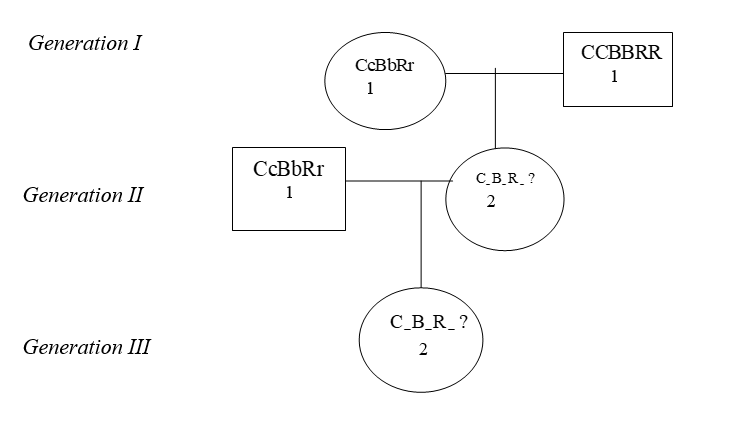
\includegraphics[height=7cm,width=11cm]{trihybrid_pedigree}
   	\caption{genetic pedigree for trihybrid Cross}
   \end{figure}
Again, our objective is to determine the probability that Generation III-2 is genotypically heterozygous curly haired, black and rough fur \textit{(CcBbRr)}. Punnett square of Generation II-2 is shown in Table 4 and for Generation III-2 is shown in table V.
\begin{figure}
	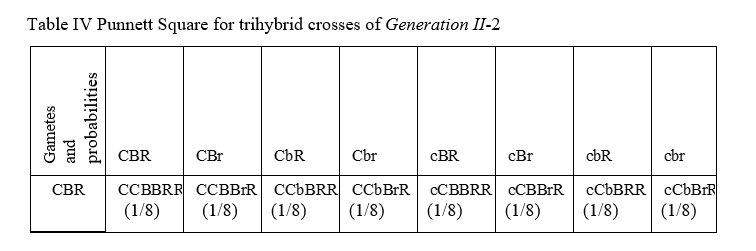
\includegraphics[height=6cm,width=18cm]{table4}\\
	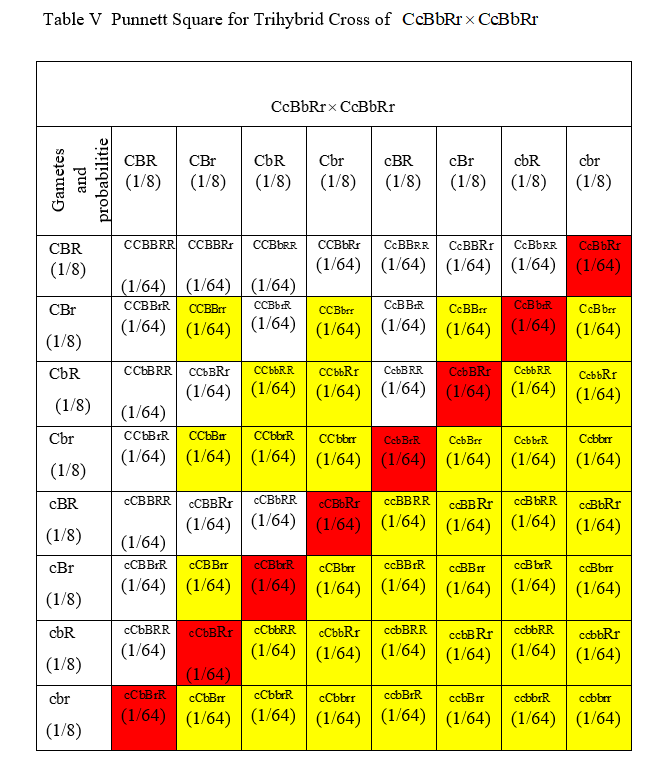
\includegraphics[height=18cm,width=16cm]{table5}
\end{figure}
From table 4 we can know the value of $ Pr(h_2|I)$ and the total prior probabilities among all possible off-spring in Generation III, producing an individual of genotype, can be kown from table V which is found by summation of all red colored rectangles labeled probabilities. All of the yellow colored-rectangles in Table V within eight Punnet Square tables are used in order to obtain normalized constant $ Pr(E|I). $\\
\begin{align*}
Pr(h_2|I) = Pr(CcBbRr|I) = \dfrac{1}{8},\hspace{6mm}   	 
\end{align*} 
Now, we find the total probability,
\begin{align*}
Pr(E|I) &= Pr(A\hspace{2mm}=\hspace{2mm}curly\hspace{2mm} hair,\hspace{2mm}black\hspace{2mm}and \hspace{2mm} rough\hspace{2mm}fur|I)\\
&= 1 - Pr(A^{T}|I)\\
&= \dfrac{343}{512}
\end{align*}
Now substituting, the above values in bayseian Equation (1), we get our required probability-
\begin{align*}
Pr(h2|E,I) &= \dfrac{Pr(h_2|I)\cdot 1}{Pr(E|I)} \\\\
Pr(h2|E,I) &= \dfrac{64}{343} 
\end{align*}
The above was the probability of hetrozygous curly haired and black and rough fur after Generation II (n=2) i.e for Generation III for trihybrid crosses.

\item \textbf{Multihybrid}\\
We found the probability of hetrozygous traits in hamster after Generation II (n=2) in dihybrid and trihybrid. If we observe the trend of praobability for n=2, in monohyrid, dihybrid and tribrid, we conclude the following-\\\\
In monohybrid, for n=2, $ Pr(h_2|E.I) = \dfrac{4}{7} $\\\\
In dihybrid, for n=2, $ Pr(h_2|E.I) = \dfrac{16}{49} = \Big(\dfrac{4}{7}\Big)^{2}  $\\\\
In trihybrid, for n=2, $ Pr(h_2|E.I) = \dfrac{64}{343} = \Big(\dfrac{4}{7}\Big)^{3} $\\\\
As we derived previously the genral exression for monohybrid cross to find the posterior PDF of $ h_2 $ for any generation n is as follows-
\begin{align*}
Pr(h_2|E,I) = \dfrac{2^n}{3\cdot 2^{n-1} + 1}
\end{align*}\\
Hence for, m different traits, we can say that-
\begin{align*}
Pr(h_2|E,I) = \Big(\dfrac{2^n}{3\cdot 2^{n-1} + 1}\Big)^{m}
\end{align*}\\

\hspace{7cm} \textit{OR}\\
\begin{align*}
Pr(h_2|E,I) =\Big(\dfrac{2^n}{3}\Big)^m \cdot \Big(\dfrac{1}{2^{n-1} + 3^{-1}}\Big)^{m}
\end{align*}
Here, we assumed the equation for posterior probability of $ h_2 $ for m different traits. We try prove the correctness of our assumption using Induction method. From equation (2), we can say that \\\\
To Prove $\Bigg(\dfrac{1/2 \cdot 1}{1 + \Big(-\dfrac{1}{8}\Big) + \Big(-\dfrac{1}{16}\Big) +.......+ \Big(-\dfrac{1}{2^{n}}\Big)}\Bigg)^{m} = \Big(\dfrac{2^n}{3\cdot 2^{n-1} + 1}\Big)^{m}$\\\\\\\\
Let P(m): $\Bigg(\dfrac{1/2 \cdot 1}{1 + \Big(-\dfrac{1}{8}\Big) + \Big(-\dfrac{1}{16}\Big) +.......+ \Big(-\dfrac{1}{2^{n}}\Big)}\Bigg)^{m} = \Big(\dfrac{2^n}{3\cdot 2^{n-1} + 1}\Big)^{m} $ \\\\
\textbf{Base case:} For m = 1 (monohybrid),
\begin{align*}
\textbf{L.H.S.} &= \Bigg(\dfrac{1/2 \cdot 1}{1 + \Big(-\dfrac{1}{8}\Big) + \Big(-\dfrac{1}{16}\Big) +.......+ \Big(-\dfrac{1}{2^{n}}\Big)}\Bigg)^{1}\\\\
&= \dfrac{1/2 \cdot 1}{1 - \Big(\dfrac{1}{8} + \dfrac{1}{16} + \dfrac{1}{32} +......+ \dfrac{1}{2^{n+1}}\Big)}\\\\  
&= \dfrac{1/2}{\dfrac{3}{4} + \dfrac{1}{2^{n+1}}} \\\\
&= \dfrac{2^n}{3\cdot 2^{n-1} + 1}\\\\
&= \textbf{R.H.S.}
\end{align*}
Hence, the equation holds true for base case i.e. monohybrid crosses (as derived earlier).\\
Now assume that this equation is true for m = k. Hence, for m = k,\\
\begin{align*}
\Bigg(\dfrac{1/2 \cdot 1}{1 + \Big(-\dfrac{1}{8}\Big) + \Big(-\dfrac{1}{16}\Big) +.......+ \Big(-\dfrac{1}{2^{n}}\Big)}\Bigg)^{k} = \Big(\dfrac{2^n}{3\cdot 2^{n-1} + 1}\Big)^{k}
\end{align*}\\
Now for m = k+1\\\\
\textbf{L.H.S.} 
\begin{align*}
&= \Bigg(\dfrac{1/2 \cdot 1}{1 + \Big(-\dfrac{1}{8}\Big) + \Big(-\dfrac{1}{16}\Big) +.....+ \Big(-\dfrac{1}{2^{n}}\Big)}\Bigg)^{k+1}\\\\
&= \Bigg(\dfrac{1/2 \cdot 1}{1 + \Big(-\dfrac{1}{8}\Big) + \Big(-\dfrac{1}{16}\Big) +..+ \Big(-\dfrac{1}{2^{n}}\Big)}\Bigg)^{k}\Bigg(\dfrac{1/2 \cdot 1}{1 + \Big(-\dfrac{1}{8}\Big) + \Big(-\dfrac{1}{16}\Big) +..+ \Big(-\dfrac{1}{2^{n}}\Big)}\Bigg)  \\ 
\end{align*}
From above assumption for n=k, we substitute the value-\\
\begin{align*}   
&= \Big(\dfrac{2^n}{3\cdot 2^{n-1} + 1}\Big)^{k}\cdot\Bigg(\dfrac{1/2 \cdot 1}{1 + \Big(-\dfrac{1}{8}\Big) + \Big(-\dfrac{1}{16}\Big) +..+ \Big(-\dfrac{1}{2^{n}}\Big)}\Bigg)\\\\   
&= \Big(\dfrac{2^n}{3\cdot 2^{n-1} + 1}\Big)^{k}\cdot \Bigg(\dfrac{1/2}{\dfrac{3}{4} + \dfrac{1}{2^{n+1}}}\Bigg)\\\\
&= \Big(\dfrac{2^n}{3\cdot 2^{n-1} + 1}\Big)^{k+1}\\\\
&= \textbf{R.H.S.}     	  
\end{align*}\\
Hence, P(K+1) is true\\\\
$ \therefore $P(1) is true and P(k) is true $ \implies $ P(K+1)is true\\\\
$ \therefore $ P(m) is true, $ \forall m \in N $ by principal of Mathematical Induction.
Hence, our above observation for calculating the probability for multihybrid crosses holds correct.
\end{itemize}

\subsubsection{New Coding / Algorithm}
We try to plot Generation vs. Posterior PDF of hetrozgous characteristics for n generation of Monhybrid, Dihybrid and Trihybrid crosses. To plot these graphs, we use the above derived equation for multihybrid by substituting the values as m = 1 (for monohybrid), m = 2 (for dihybrid) and m = 3 (for trihybrid).\\ From the plot given in figure 7 we observe that as $ n \rightarrow \infty $, $ Pr(h_2|E,I) $ approaches 0.666 in monohybrid, in dihybrid it approaches to 0.444 and in trihybrid it approahes to 0.2963 \\\\
\begin{figure}[h]
	\centering
	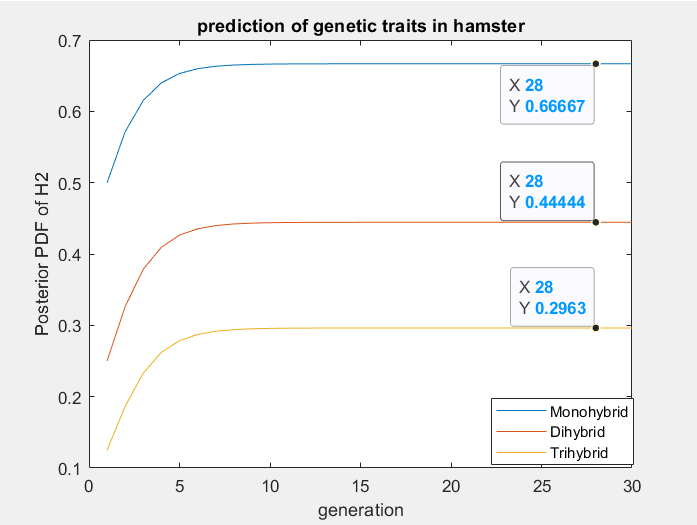
\includegraphics[height=11cm,width=13cm]{code2}
	\caption{Probability of hetrozygous characteristics in monohybrid, dihybrid and trihybrid}
\end{figure}

\section{Inference Analysis}
	
\begin{itemize}
	
\item In this study, we predicted the probability of transmission of genetic traits from generation to generation within a Bayesian framework and developed a mathematical code that calculates posterior probability of hypothesis for genetic crossing of traits. We extended the study to calculate the probability for multihybrid species. We implemened this trivial experiment to find different characteristic of hamster.

\item Further, this can model the trend of transmission of autosomal recessive disesases like Cystic Fibrosis (CF). Under assumption that any person being CF patient and all crossings
with him/her and next generations after him/her are not affected by phenotypically CF disease. We can find the probability that his child, grandson and so on are being genetically either heterozygous or homozygous. 

\end{itemize} 

\section{ Contribution of team members}	
\subsection{Technical contribution of all team members }
\begin{table}[h]
	\centering
	\begin{tabular}{|l|l|l|l|}
		\hline
		Tasks  & Nancy Radadia & Suhanee Patel & Yash Patel      \\ \hline
		Concept Maps & \hspace{1cm}$ \checkmark $&       \hspace{1cm}$ \checkmark $        &     \hspace{0.7cm}$ \checkmark $            \\ \hline
		Data Scraping &    \hspace{1cm}$ \checkmark $           &     \hspace{1cm}$ \checkmark $          &      \hspace{0.7cm}$ \checkmark $         \\ \hline
		Latex Coding &   \hspace{1cm}$ \checkmark $            &   \hspace{1cm}$ \checkmark $             &  \hspace{0.7cm}$ \checkmark $              \\ \hline
		Coding in Matlab &  \hspace{1cm}$ \checkmark $              &   \hspace{1cm}$ \checkmark $ &  \hspace{0.7cm}$ \checkmark $              \\ \hline
		References and Conclusions & \hspace{1cm}$ \checkmark $ & \hspace{1cm}$ \checkmark $              &    \hspace{0.7cm}$ \checkmark $           \\ \hline
	\end{tabular}
\end{table}
\subsection{Non-Technical contribution of all team members }
\begin{table}[h]
\centering
\begin{tabular}{|l|l|l|l|}
\hline
Tasks  & Nancy Radadia & Suhanee Patel & Yash Patel      \\ \hline
Report Writing & \hspace{1cm}$ \checkmark $&       \hspace{1cm}$ \checkmark $        &     \hspace{0.7cm}$ \checkmark $            \\ \hline
Web Surfing &    \hspace{1cm}$ \checkmark $           &     \hspace{1cm}$ \checkmark $          &      \hspace{0.7cm}$ \checkmark $         \\ \hline
Latex Coding &   \hspace{1cm}$ \checkmark $            &               &               \\ \hline
Reviewing Article &               &        \hspace{1cm}$ \checkmark $       &               \\ \hline
References and editing Article &               &               &    \hspace{0.7cm}$ \checkmark $           \\ \hline
\end{tabular}
\end{table}

%\vspace{0.5cm}

\bibliographystyle{IEEEtran}
\bibliography{ref.bib}

\end{document} 